\documentclass[conference]{IEEEtran}

% ========================
% PACOTES
% ========================
\usepackage[utf8]{inputenc}
\usepackage[T1]{fontenc}
\usepackage[brazilian]{babel}
\usepackage{cite}
\usepackage{amsmath,amssymb}
\usepackage{graphicx}
\usepackage{url}
\usepackage{hyperref}
\hypersetup{colorlinks=true, linkcolor=red, citecolor=red, urlcolor=red}
\usepackage{booktabs}
\usepackage{algorithm}
\usepackage{algorithmic}
\usepackage{acronym}
\usepackage{xcolor}
\usepackage{listings}
\usepackage{multirow}
\usepackage{tabularx}
\usepackage{enumitem}

% Nomes em português para algoritmos
\floatname{algorithm}{Algoritmo}
\renewcommand{\algorithmicrequire}{\textbf{Entrada:}}
\renewcommand{\algorithmicensure}{\textbf{Saída:}}
\renewcommand{\algorithmicfor}{\textbf{para}}
\renewcommand{\algorithmicdo}{\textbf{faça}}
\renewcommand{\algorithmicend}{\textbf{fim}}
\renewcommand{\algorithmicif}{\textbf{se}}
\renewcommand{\algorithmicthen}{\textbf{então}}
\renewcommand{\algorithmicelse}{\textbf{senão}}
\renewcommand{\algorithmicreturn}{\textbf{retorne}}
\renewcommand{\algorithmicwhile}{\textbf{enquanto}}
\renewcommand{\algorithmicrepeat}{\textbf{repita}}
\renewcommand{\algorithmicuntil}{\textbf{até}}

\renewcommand{\IEEEkeywordsname}{Palavras-chave}

% ========================
% DOCUMENTO
% ========================
\begin{document}

\title{{Otimização da Eficiência de Rede Assistida por Aprendizado Federado Usando IA Generativa e Imagens}
\thanks{
%This work was supported in part by the Coordenação de Aperfeiçoamento de Pessoal de Nível Superior - Brasil (CAPES) – PDSE Program and by the National Council for Scientific and Technological Development (CNPq) of Brazil under Grants 405301/2021-9, 141485/2020-5, and 310681/2019-7. The work of M. V. Vejling and P. Popovski were supported in part by the Villum Investigator Grant "WATER" financed by the VILLUM Foundation, Denmark.
}
}
\author{
\IEEEauthorblockN{
    {%\hs
    {Gian Pedro Rodrigues}}\IEEEauthorrefmark{1},
    {%\mv
    {Herman L. dos Santos}}\IEEEauthorrefmark{1},%\IEEEauthorrefmark{3},
    % {%\ta
    % {~}}\IEEEauthorrefmark{1},
    % and {%\pp
    % {~}}\IEEEauthorrefmark{2} \\
        }
        \IEEEauthorblockA{
        \IEEEauthorrefmark{1}\textit{\small Departamento Academico de Engenharia Elétrica, Universidade Tecnológica Federal do Paraná}, Cornélio Procópio, Brasil\\
        %\IEEEauthorrefmark{2}\textit{\small Department of Electronic Systems, Aalborg University}, Aalborg, Denmark\\
        %\IEEEauthorrefmark{3}\textit{\small Department of Mathematical Sciences, Aalborg University}, Aalborg, Denmark\\
        \small E-mail: hermansantos@utfpr.edu.br, gian.2000@alunos.utfpr.edu.br% mvv@es.aau.dk, taufik@uel.br, and petarp@es.aau.dk
        }
}

\maketitle

% ========================
% RESUMO
% ========================
\begin{abstract}
Este trabalho apresenta um framework containerizado para investigar a comunicação semântica de imagens utilizando aprendizado federado e IA generativa. O sistema emprega tanto um autoencoder convolucional determinístico quanto um \textit{Variational Autoencoder} (VAE) — modelo genuinamente generativo — treinados de forma distribuída entre múltiplos dispositivos simulados por contêineres Docker. Ambos os modelos comprimem imagens do dataset MNIST de 784 pixels para apenas 32 valores no espaço latente (redução de 96\%), sendo que o VAE aprende uma distribuição contínua no espaço latente capaz de gerar novas imagens sem precedentes nos dados de treinamento. O treinamento federado utiliza o algoritmo FedAvg com compressão Top-K dos pesos do modelo, enquanto um mecanismo de injeção de caos baseado em \texttt{tc netem} avalia a resiliência sob condições adversas de rede. Adicionalmente, o sistema incorpora simulação de canal AWGN no espaço latente, aproximando-se de um esquema de codificação conjunta fonte-canal (JSCC). Os resultados demonstram: (i) a viabilidade da comunicação semântica generativa via FL; (ii) a superioridade do treinamento centralizado sobre o federado em qualidade pura, evidenciando o trade-off com privacidade; (iii) a robustez do framework sob quatro cenários de caos; e (iv) a capacidade de completação de imagens parciais e geração de novas amostras pelo VAE.
\end{abstract}

\begin{IEEEkeywords}
Aprendizado Federado, Comunicação Semântica, IA Generativa, Variational Autoencoder, Docker, Injeção de Caos, JSCC, SSIM
\end{IEEEkeywords}

% ========================
% ACRÔNIMOS
% ========================
\input{acronym}

% ========================
% SEÇÃO 1: INTRODUÇÃO
% ========================
\section{Introdução}

O crescimento exponencial de dispositivos conectados na Internet das Coisas (IoT) e o avanço das redes sem fio 5G/6G têm gerado desafios significativos em termos de largura de banda, latência e privacidade \cite{kairouz2021advances}. Sistemas tradicionais de comunicação, fundamentados na teoria de Shannon \cite{shannon1948}, focam em transmitir bits com máxima fidelidade, ignorando o \textit{significado} da informação. Por exemplo, ao transmitir uma imagem de um dígito manuscrito, o sistema clássico precisa enviar todos os 784 pixels, mesmo que a informação semântica possa ser representada de forma muito mais compacta.

Nesse contexto, a \textbf{comunicação semântica} surge como paradigma promissor: o transmissor extrai a essência da informação e envia uma representação compacta ao receptor, que reconstrói a mensagem original \cite{xie2021deep, yang2022semantic}. Recentemente, modelos de \textbf{IA generativa} — como \ac{VAE}s, GANs e modelos de difusão — têm sido propostos como codecs semânticos avançados, capazes não apenas de comprimir, mas de \textit{gerar} conteúdo semanticamente coerente no receptor \cite{grassucci2023genai_meets_semcom, du2023genainet}. Paralelamente, o \textbf{\ac{FL}} consolidou-se como abordagem para treinar modelos de forma descentralizada, onde cada dispositivo treina localmente e compartilha apenas os parâmetros do modelo — nunca os dados brutos \cite{mcmahan2017}.

A combinação dessas tecnologias permite que dispositivos distribuídos colaborem no treinamento de um codec semântico generativo sem compartilhar dados privados. Este trabalho propõe um \textbf{testbed prático e reprodutível} que integra essas abordagens, utilizando contêineres Docker para simular um cenário distribuído. Dois modelos são avaliados: um \textbf{autoencoder convolucional} determinístico e um \textbf{Variational Autoencoder (VAE)} — modelo genuinamente generativo \cite{kingma2014vae} — que aprende uma distribuição no espaço latente, permitindo geração de novas amostras e comunicação semântica mais robusta. Ambos comprimem imagens MNIST para um vetor de 32 dimensões (compressão de 96\%), e permitem testar a \textbf{completação de imagens parciais}. Adicionalmente, o sistema incorpora simulação de canal \ac{AWGN} no espaço latente, aproximando o conceito de codificação conjunta fonte-canal (\ac{JSCC}) \cite{bourtsoulatze2019deep}.

As principais contribuições deste trabalho são:

\begin{itemize}[leftmargin=*]
    \item Um framework containerizado e reprodutível para treinamento federado e comunicação semântica generativa de imagens, orquestrado via Docker Compose;
    \item Um \ac{VAE} como codec semântico generativo, capaz de comprimir, reconstruir e \textit{gerar} novas imagens a partir de uma distribuição aprendida no espaço latente \cite{kingma2014vae};
    \item Comparação sistemática entre AE determinístico e VAE generativo, e entre treinamento centralizado e federado, evidenciando trade-offs de qualidade vs. privacidade;
    \item Simulação de canal \ac{AWGN} no espaço latente, aproximando o conceito de \ac{JSCC};
    \item Compressão Top-K dos pesos do modelo (60\% de esparsidade) para reduzir o custo de comunicação durante o treinamento federado;
    \item Avaliação com métricas MSE, PSNR e \ac{SSIM} \cite{wang2004ssim}, alinhada ao estado da arte em comunicação semântica;
    \item Um mecanismo configurável de injeção de caos baseado em \texttt{tc netem} para avaliar a robustez do sistema sob condições adversas.
\end{itemize}

O restante do artigo está organizado da seguinte forma: a Seção~\ref{sec:related} apresenta os trabalhos relacionados; a Seção~\ref{sec:system} descreve a arquitetura proposta em detalhes; a Seção~\ref{sec:results} apresenta os resultados experimentais; e a Seção~\ref{sec:conclusion} conclui o trabalho com discussões e direções futuras.


% ========================
% SEÇÃO 2: TRABALHOS RELACIONADOS
% ========================
\section{Trabalhos Relacionados}
\label{sec:related}

\subsection{Aprendizado Federado}

O \ac{FL} foi formalizado por McMahan et al. \cite{mcmahan2017}, que propuseram o FedAvg para agregar modelos treinados localmente. Cada dispositivo treina uma cópia local e envia apenas os pesos ao servidor, que calcula a média dos parâmetros. Diversas extensões abordaram desafios como dados heterogêneos (non-IID) \cite{zhao2018federated}, compressão de gradientes \cite{konevcny2016federated} e robustez contra falhas \cite{blanchard2017machine}. Li et al. \cite{li2020federated} e Kairouz et al. \cite{kairouz2021advances} compilaram os principais avanços e problemas em aberto, destacando a necessidade de compressão eficiente para cenários com largura de banda limitada.

\subsection{Comunicação Semântica}

A comunicação semântica, inspirada nos três níveis de comunicação de Shannon e Weaver \cite{shannon1948}, ganhou impulso com deep learning. Yang et al. \cite{yang2022semantic} revisaram fundamentos e desafios, apontando autoencoders como arquitetura promissora. O DeepSC \cite{xie2021deep} utilizou redes neurais para codificação semântica de texto. Bourtsoulatze et al. \cite{bourtsoulatze2019deep} propuseram autoencoders para \ac{JSCC} de imagens, demonstrando que redes neurais podem superar esquemas tradicionais em baixa relação sinal-ruído. Weng e Qin \cite{weng2021semantic} estenderam a abordagem para sinais de fala. Luo et al. \cite{luo2022semantic} destacaram a necessidade de testbeds práticos, e Kurka e Gündüz \cite{eirina2019deep} propuseram o DeepJSCC-f com feedback de canal.

\subsection{IA Generativa para Comunicação Semântica}

Recentemente, modelos generativos emergiram como evolução natural dos codecs semânticos baseados em autoencoders determinísticos. Grassucci et al. \cite{grassucci2023genai_meets_semcom} apresentaram uma taxonomia abrangente dos modelos generativos — \ac{VAE}s, GANs e modelos de difusão — aplicados à comunicação semântica, destacando que modelos generativos permitem não apenas comprimir, mas \textit{gerar} conteúdo no receptor a partir de uma descrição semântica compacta. Du et al. \cite{du2023genai_semcom} propuseram o uso de modelos de difusão para comunicação semântica sem necessidade de treinamento conjunto transmissor-receptor.

No contexto de redes wireless, Du et al. \cite{du2023genainet} introduziram o GenAINet, um framework que utiliza IA generativa para inteligência coletiva em redes sem fio, propondo mecanismos de transferência de conhecimento e raciocínio no edge. Xia et al. \cite{xia2023gennet_layer} formalizaram a \textit{camada generativa de rede}, posicionando o modelo generativo como componente integral do protocolo de comunicação, capaz de adaptar-se dinamicamente às condições do canal.

O \ac{VAE}, proposto por Kingma e Welling \cite{kingma2014vae}, é particularmente adequado para comunicação semântica por aprender uma distribuição contínua no espaço latente $p(z) = \mathcal{N}(0, I)$, o que confere regularidade ao espaço de representações e permite geração de novas amostras. Higgins et al. \cite{higgins2017beta_vae} introduziram o $\beta$-VAE, onde o hiperparâmetro $\beta$ controla o trade-off entre qualidade de reconstrução e regularidade do espaço latente — conceito diretamente relevante para comunicação, onde o espaço latente funciona como canal de transmissão.

Neste trabalho, posicionamos nosso framework no contexto dessas referências: implementamos e comparamos um AE determinístico com um VAE generativo, ambos treinados via FL, com simulação de canal AWGN — abordando lacunas identificadas na literatura recente.

\subsection{Testbeds e Engenharia de Caos}

A maioria dos trabalhos na área utiliza simulações idealizadas, sem imperfeições reais de rede. O conceito de \textbf{engenharia de caos}, popularizado pela Netflix \cite{basiri2016chaos}, consiste em introduzir falhas intencionais para avaliar a resiliência de um sistema. A ferramenta \texttt{tc netem} do Linux permite simular perda de pacotes, latência e corrupção em interfaces de rede reais. Neste trabalho, aplicamos esse conceito ao treinamento federado, executando comunicação real entre processos isolados com injeção de imperfeições configuráveis em tempo real.


% ========================
% SEÇÃO 3: SISTEMA PROPOSTO
% ========================
\section{Sistema Proposto}
\label{sec:system}

Nesta seção, descrevemos cada componente do framework proposto.

\subsection{Visão Geral da Arquitetura}

O sistema é composto por cinco contêineres Docker orquestrados via Docker Compose. Cada contêiner simula um componente de um sistema distribuído de comunicação, conforme descrito na Tabela~\ref{tab:containers}.

\begin{table}[h]
\centering
\caption{Contêineres do sistema e suas funções}
\label{tab:containers}
\begin{tabular}{lp{5.0cm}}
\toprule
\textbf{Contêiner} & \textbf{Função} \\
\midrule
\texttt{fl-server} & Servidor Flask que recebe pesos dos clientes, executa agregação FedAvg e disponibiliza o modelo global via API REST \\
\texttt{client-full} & Cliente estável que treina com todos os dígitos (IID) e envia pesos completos (sem compressão) \\
\texttt{client-noisy} & Cliente instável que aplica compressão Top-K (60\% esparsidade) antes de enviar os pesos \\
\texttt{client-noniid} & Cliente com dados heterogêneos (Non-IID), treinando apenas com os dígitos 0--3, enviando pesos completos \\
\texttt{dashboard} & Painel Streamlit para visualização em tempo real, testes interativos de comunicação semântica e controle do caos \\
\texttt{chaos-injector} & Contêiner Alpine que aplica regras \texttt{tc netem} na interface de rede do cliente instável \\
\bottomrule
\end{tabular}
\end{table}

Os contêineres compartilham a mesma imagem Docker (Python 3.9 + PyTorch) e comunicam-se via rede bridge \texttt{fl-network}, usando nomes de serviços como hostnames. O injetor de caos opera no namespace de rede do cliente instável (via \texttt{network\_mode: service:client-noisy}), permitindo que regras \texttt{tc netem} afetem diretamente o tráfego desse contêiner.

A inclusão de três clientes com perfis distintos permite uma avaliação mais realista do treinamento federado: o \texttt{client-full} serve como baseline estável; o \texttt{client-noisy} testa a resiliência à compressão e caos de rede; e o \texttt{client-noniid} avalia o impacto de dados heterogêneos (Non-IID) na convergência do modelo global, um dos principais desafios em FL \cite{zhao2018federated}.

\subsection{Comunicação entre Contêineres}

A comunicação é realizada via \textbf{API REST} (HTTP). O servidor Flask expõe quatro endpoints: \texttt{POST /upload} para receber pesos treinados; \texttt{GET /global\_model} para distribuir o modelo global; \texttt{POST /reconstruct} para decodificar um vetor latente em imagem; e \texttt{POST /complete} para reconstruir uma imagem parcial. Essa arquitetura é extensível — novos clientes são adicionados configurando um contêiner que aponte para o servidor.

\subsection{Autoencoder Convolucional}

O modelo central do sistema é um autoencoder convolucional projetado para comprimir e reconstruir imagens MNIST (1$\times$28$\times$28 pixels). O autoencoder é composto por duas partes simétricas: o encoder (compressor) e o decoder (reconstrutor).

O encoder comprime a imagem (28$\times$28 pixels) para um vetor latente de 32 dimensões através de duas camadas convolucionais com ReLU e max-pooling, seguidas de duas camadas totalmente conectadas (3136$\rightarrow$256$\rightarrow$32). O decoder realiza o caminho inverso, expandindo o vetor latente via camadas lineares e convolução transposta com ativação Sigmoid final. A Tabela~\ref{tab:architecture} detalha a arquitetura completa.

\begin{table}[h]
\centering
\caption{Arquitetura detalhada do autoencoder convolucional}
\label{tab:architecture}
\begin{tabular}{llr}
\toprule
\textbf{Camada} & \textbf{Tipo} & \textbf{Saída} \\
\midrule
\multicolumn{3}{c}{\textit{Encoder}} \\
\midrule
Entrada & Imagem & 1$\times$28$\times$28 \\
Conv2d + ReLU & 32 filtros, 3$\times$3 & 32$\times$28$\times$28 \\
MaxPool2d & 2$\times$2 & 32$\times$14$\times$14 \\
Conv2d + ReLU & 64 filtros, 3$\times$3 & 64$\times$14$\times$14 \\
MaxPool2d & 2$\times$2 & 64$\times$7$\times$7 \\
Flatten + Linear & 3136 $\rightarrow$ 256 & 256 \\
Linear & 256 $\rightarrow$ 32 & \textbf{32} \\
\midrule
\multicolumn{3}{c}{\textit{Decoder}} \\
\midrule
Linear & 32 $\rightarrow$ 256 & 256 \\
Linear & 256 $\rightarrow$ 3136 & 3136 \\
Reshape & --- & 64$\times$7$\times$7 \\
ConvTranspose2d + ReLU & 32 filtros & 32$\times$14$\times$14 \\
ConvTranspose2d + Sigmoid & 1 filtro & 1$\times$28$\times$28 \\
\bottomrule
\end{tabular}
\end{table}

A função de perda utilizada para treinamento é o \ac{MSE}:

\begin{equation}
\mathcal{L}_{\text{MSE}} = \frac{1}{N} \sum_{i=1}^{N} \| \mathbf{x}_i - \hat{\mathbf{x}}_i \|^2
\label{eq:mse}
\end{equation}

\noindent onde $\mathbf{x}_i$ é a imagem original e $\hat{\mathbf{x}}_i$ é a imagem reconstruída pelo decoder. Essa função penaliza diferenças pixel a pixel entre a entrada e a saída, incentivando o modelo a preservar os detalhes visuais.

A taxa de compressão alcançada pelo codec semântico é:

\begin{equation}
R_c = 1 - \frac{D_{\text{latente}}}{D_{\text{original}}} = 1 - \frac{32}{784} \approx 95{,}9\%
\label{eq:compression}
\end{equation}

\noindent Isso significa que mais de 95\% dos dados podem ser descartados durante a transmissão, enviando-se apenas 32 números reais em vez de 784 pixels.

\subsection{Variational Autoencoder (VAE) como Codec Generativo}

Embora o autoencoder determinístico comprima eficientemente, ele não é um modelo generativo — não permite amostrar novas imagens do espaço latente. Para incorporar IA generativa ao framework, implementamos um \ac{VAE} \cite{kingma2014vae} como alternativa ao AE.

O VAE utiliza o mesmo backbone convolucional (encoder e decoder), com a diferença fundamental de que a última camada do encoder é bifurcada em duas cabeças: $\boldsymbol{\mu}$ (média) e $\log \boldsymbol{\sigma}^2$ (log-variância), produzindo uma distribuição posterior $q(\mathbf{z}|\mathbf{x}) = \mathcal{N}(\boldsymbol{\mu}, \boldsymbol{\sigma}^2 \mathbf{I})$. A amostragem utiliza o \textit{reparameterization trick} \cite{kingma2014vae}:

\begin{equation}
\mathbf{z} = \boldsymbol{\mu} + \boldsymbol{\sigma} \odot \boldsymbol{\epsilon}, \quad \boldsymbol{\epsilon} \sim \mathcal{N}(\mathbf{0}, \mathbf{I})
\label{eq:reparam}
\end{equation}

A função de perda do VAE combina reconstrução e regularização:

\begin{equation}
\mathcal{L}_{\text{VAE}} = \underbrace{\mathcal{L}_{\text{MSE}}}_{\text{reconstrução}} + \beta \cdot \underbrace{D_{\text{KL}}\big(q(\mathbf{z}|\mathbf{x}) \,\|\, \mathcal{N}(\mathbf{0}, \mathbf{I})\big)}_{\text{regularização}}
\label{eq:vae_loss}
\end{equation}

\noindent onde a divergência \ac{KL} tem forma analítica:

\begin{equation}
D_{\text{KL}} = -\frac{1}{2} \sum_{j=1}^{d} \left(1 + \log \sigma_j^2 - \mu_j^2 - \sigma_j^2\right)
\label{eq:kl}
\end{equation}

O hiperparâmetro $\beta$ (conceito de $\beta$-VAE \cite{higgins2017beta_vae}) controla o trade-off entre fidelidade de reconstrução e regularidade do espaço latente: $\beta > 1$ favorece um espaço latente mais organizado (útil para geração), enquanto $\beta < 1$ prioriza reconstrução. Neste trabalho, utilizamos $\beta = 1$ (VAE padrão).

A principal vantagem do VAE para comunicação semântica é que o espaço latente regularizado $p(\mathbf{z}) = \mathcal{N}(\mathbf{0}, \mathbf{I})$ permite: (i) \textit{geração} — novas imagens são criadas amostrando $\mathbf{z} \sim \mathcal{N}(\mathbf{0}, \mathbf{I})$ e decodificando; (ii) \textit{robustez ao canal} — a regularidade do espaço latente torna a representação mais tolerante a perturbações; e (iii) \textit{interpolação} — transições suaves entre representações semânticas no espaço latente. A Tabela~\ref{tab:ae_vs_vae_arch} resume as diferenças arquiteturais.

\begin{table}[ht]
\centering
\caption{Comparação arquitetural AE vs. VAE}
\label{tab:ae_vs_vae_arch}
\begin{tabular}{lcc}
\toprule
\textbf{Característica} & \textbf{AE} & \textbf{VAE} \\
\midrule
Encoder saída & Vetor $\mathbf{z} \in \mathbb{R}^{32}$ & $\boldsymbol{\mu}, \log\boldsymbol{\sigma}^2 \in \mathbb{R}^{32}$ \\
Espaço latente & Determinístico & Probabilístico \\
Loss & MSE & MSE + $\beta \cdot$ KL \\
Generativo & Não & Sim \\
Parâmetros & 1.663.265 & 1.671.489 \\
\bottomrule
\end{tabular}
\end{table}

\subsection{Modelo de Canal AWGN no Espaço Latente}

Para aproximar o cenário real de comunicação wireless, incorporamos um modelo de canal \ac{AWGN} diretamente no espaço latente, seguindo a abordagem de \ac{JSCC} proposta por Bourtsoulatze et al. \cite{bourtsoulatze2019deep}. Durante o treinamento, o vetor latente é corrompido por ruído gaussiano antes da decodificação:

\begin{equation}
\hat{\mathbf{z}} = \mathbf{z} + \mathbf{n}, \quad \mathbf{n} \sim \mathcal{N}\left(\mathbf{0}, \sigma_n^2 \mathbf{I}\right)
\label{eq:awgn}
\end{equation}

\noindent onde $\sigma_n = 1/\sqrt{10^{\text{SNR}_{\text{dB}}/10}}$. Ao treinar com o canal AWGN ativo, o modelo aprende representações latentes mais robustas a perturbações, efetivamente realizando codificação conjunta fonte-canal: o encoder atua simultaneamente como compressor semântico e codificador de canal, enquanto o decoder realiza decodificação conjunta.

\subsection{Métricas de Avaliação}

Além do \ac{MSE} (Eq.~\ref{eq:mse}) e do \ac{PSNR}, este trabalho emprega o \ac{SSIM} \cite{wang2004ssim}, métrica padrão na literatura de comunicação semântica que avalia a similaridade estrutural entre imagens:

\begin{equation}
\text{SSIM}(\mathbf{x}, \hat{\mathbf{x}}) = \frac{(2\mu_x \mu_{\hat{x}} + C_1)(2\sigma_{x\hat{x}} + C_2)}{(\mu_x^2 + \mu_{\hat{x}}^2 + C_1)(\sigma_x^2 + \sigma_{\hat{x}}^2 + C_2)}
\label{eq:ssim}
\end{equation}

\noindent O SSIM captura similaridade de luminância, contraste e estrutura, com valor 1 indicando imagens idênticas. Diferentemente do MSE (puramente pixel a pixel), o SSIM correlaciona-se melhor com a percepção humana de qualidade visual.

\subsection{Protocolo de Treinamento Federado}

O treinamento é realizado de forma distribuída utilizando o algoritmo FedAvg \cite{mcmahan2017}. O Algoritmo~\ref{alg:fedavg} descreve o protocolo completo.

\begin{algorithm}[h]
\caption{Treinamento Federado com FedAvg e Top-K}
\label{alg:fedavg}
\begin{algorithmic}[1]
\REQUIRE Servidor $S$, clientes $\{C_1, C_2, C_3\}$, rodadas $T$
\ENSURE Modelo global $\mathbf{w}^{(T)}$
\STATE Inicializar $\mathbf{w}^{(0)}$ aleatoriamente no servidor
\FOR{$t = 0$ \textbf{até} $T-1$}
    \STATE $S$ disponibiliza $\mathbf{w}^{(t)}$
    \FOR{\textbf{cada} cliente $k \in \{1, 2, 3\}$ \textbf{em paralelo}}
        \STATE $C_k$ obtém $\mathbf{w}^{(t)}$ do servidor
        \STATE $C_k$ treina localmente por 5 épocas
        \IF{$C_k$ é cliente instável}
            \STATE Aplica compressão Top-K (40\% dos pesos)
        \ENDIF
        \IF{$C_k$ é cliente Non-IID}
            \STATE Treina apenas com subconjunto de classes (dígitos 0--3)
        \ENDIF
        \STATE $C_k$ envia $\mathbf{w}_k^{(t+1)}$ ao servidor
    \ENDFOR
    \STATE $S$ agrega: $\mathbf{w}^{(t+1)} = \frac{1}{K} \sum_{k=1}^{K} \mathbf{w}_k^{(t+1)}$
\ENDFOR
\end{algorithmic}
\end{algorithm}

A cada rodada, os clientes treinam localmente por 5 épocas (batch=32, Adam, lr=0,001) e enviam os pesos ao servidor, que os agrega pela média com $K=3$ clientes. O \texttt{client-noisy} aplica \textbf{compressão Top-K}: apenas 40\% dos pesos são enviados, e os restantes são reconstruídos no servidor por \textit{imputação pela média}. O \texttt{client-noniid} treina apenas com dígitos 0--3, simulando heterogeneidade de dados (non-IID) \cite{li2020federated}.

\subsection{Comunicação Semântica de Imagens}

O sistema implementa dois modos de teste de comunicação semântica, ambos acessíveis interativamente pelo painel de visualização:

\textbf{Modo Compressão:} O transmissor codifica a imagem via encoder, obtendo um vetor latente de 32 dimensões que é transmitido ao receptor. Este utiliza o decoder para reconstruir a imagem original, avaliando a qualidade em termos de MSE, PSNR e SSIM.

\textbf{Modo Completação:} O transmissor envia apenas uma fração da imagem original, com três tipos de mascaramento: metade inferior zerada (transmissão interrompida), pixels aleatórios zerados (perda de dados) ou metade direita zerada (informação espacial parcial). O modelo reconstrói a imagem completa, incluindo a parte mascarada, demonstrando que aprendeu uma representação semântica capaz de inferir conteúdo visual faltante.

\textbf{Modo Geração (apenas VAE):} Ao utilizar o VAE, o sistema permite gerar novas imagens sem precedentes nos dados de treinamento, amostrando $\mathbf{z} \sim \mathcal{N}(\mathbf{0}, \mathbf{I})$ e decodificando. Essa capacidade demonstra que o modelo é genuinamente generativo — diferentemente do AE determinístico, que apenas reconstrói exemplos observados.

\subsection{Injeção de Caos}

O mecanismo de injeção de caos utiliza a ferramenta \texttt{tc netem} do kernel Linux para alterar dinamicamente as condições de rede do cliente instável. O contêiner \texttt{chaos-injector} executa um loop shell que lê continuamente um arquivo de configuração (\texttt{chaos\_config.txt}) e aplica as regras correspondentes na interface de rede \texttt{eth0}.

Quatro parâmetros são configuráveis em tempo real: \textbf{perda de pacotes} (0--5\%), \textbf{latência} (0--2000~ms), \textbf{corrupção} (0--2\%) e \textbf{duplicação} (0--5\%). Essas condições afetam exclusivamente o cliente instável, permitindo comparação direta com os clientes estável e Non-IID sob condições ideais.

\subsection{Painel de Visualização}

O painel Streamlit oferece seis abas para monitoramento em tempo real: \textit{Arquitetura} (topologia e perfis dos clientes), \textit{Comunicação} (teste de reconstrução semântica com métricas), \textit{Completação} (teste com imagens parciais), \textit{Terminais} (logs do servidor e clientes), \textit{Métricas} (curvas de convergência por rodada) e \textit{Experimentos} (comparação entre cenários de caos). A barra lateral controla o treinamento (play/pause) e os parâmetros de caos.


% ========================
% SEÇÃO 4: RESULTADOS
% ========================
\section{Resultados Experimentais}
\label{sec:results}

Nesta seção, apresentamos os resultados da avaliação experimental do framework proposto. Os experimentos abrangem a convergência do treinamento federado, a qualidade da reconstrução semântica, os testes de completação de imagens parciais e o impacto da injeção de caos.

\subsection{Configuração Experimental}

Os experimentos foram conduzidos utilizando Docker Desktop em ambiente local com Windows. O dataset utilizado é o MNIST \cite{lecun1998gradient}, um benchmark amplamente adotado na comunidade de aprendizado de máquina, contendo 60.000 imagens de treinamento e 10.000 de teste. Cada imagem representa um dígito manuscrito (0--9) em escala de cinza com resolução 28$\times$28 pixels. A Tabela~\ref{tab:params} apresenta os principais parâmetros do sistema.

\begin{table}[h]
\centering
\caption{Parâmetros experimentais}
\label{tab:params}
\begin{tabular}{ll}
\toprule
\textbf{Parâmetro} & \textbf{Valor} \\
\midrule
Dataset & MNIST (28$\times$28, 1 canal) \\
Imagens de treinamento & 60.000 \\
Imagens de teste & 10.000 \\
Dimensão latente & 32 \\
Pixels por imagem & 784 \\
Taxa de compressão & 95,9\% \\
Fator de compressão & 24,5$\times$ \\
Épocas locais por rodada & 5 \\
Tamanho do batch & 32 imagens \\
Otimizador & Adam (lr = 0,001) \\
Esparsidade Top-K (noisy) & 60\% \\
Número de clientes & 3 \\
Cliente Non-IID & Dígitos 0--3 \\
Modelos avaliados & AE e VAE ($\beta=1$) \\
Canal AWGN & SNR = $\{5, 10, 15, 20\}$ dB \\
Métricas & MSE, PSNR, SSIM \\
Framework ML & PyTorch 2.x \\
Contêineres & 6 (Docker Compose) \\
\bottomrule
\end{tabular}
\end{table}

\subsection{Convergência do Treinamento Federado}

A primeira análise diz respeito à convergência do treinamento federado ao longo das rodadas. A Figura~\ref{fig:convergence} apresenta a evolução da loss (MSE) para os três clientes durante o treinamento.

\begin{figure}[h]
\centering
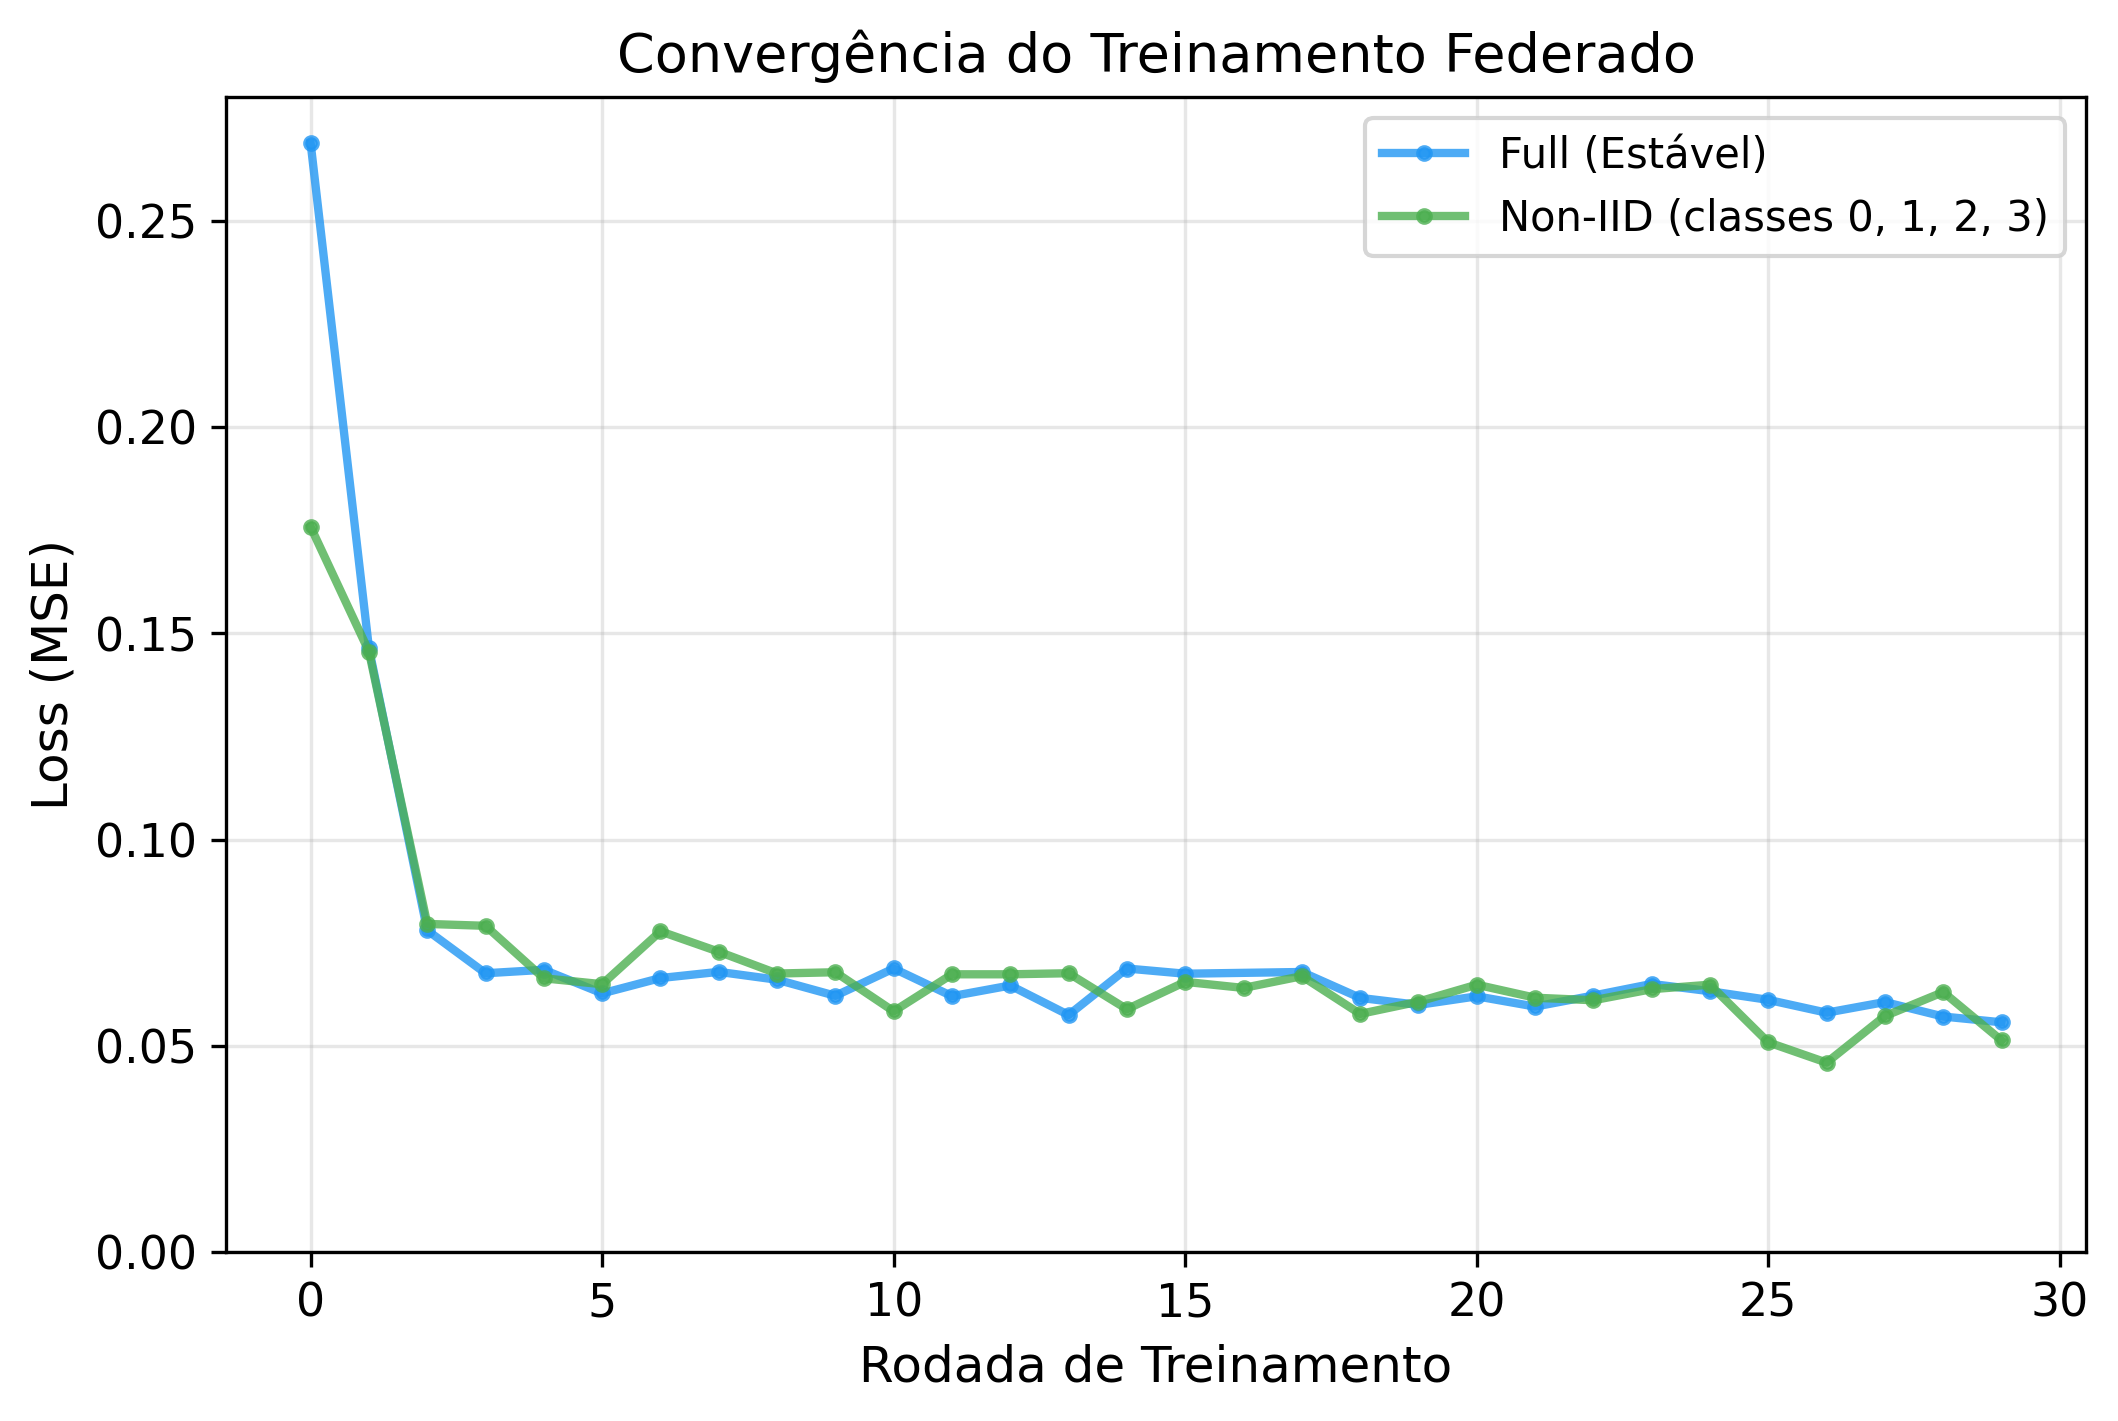
\includegraphics[width=\linewidth]{figures/fig_convergence.png}
\caption{Evolução da loss (MSE) ao longo das rodadas de treinamento federado para os três clientes: \texttt{client-full} (azul), \texttt{client-noisy} (laranja) e \texttt{client-noniid} (verde).}
\label{fig:convergence}
\end{figure}

Os resultados mostram que os três clientes apresentam convergência progressiva ao longo das rodadas. O \texttt{client-full}, com dados IID e pesos completos, converge de forma mais rápida e estável. O \texttt{client-noisy} apresenta convergência mais ruidosa devido à compressão Top-K e às condições adversas de rede. O \texttt{client-noniid} demonstra uma tendência de convergência intermediária: apesar de enviar pesos completos, a distribuição enviesada de dados (apenas dígitos 0--3) resulta em gradientes que não representam a distribuição completa dos dados, afetando a contribuição para o modelo global. A agregação FedAvg, ao calcular a média dos pesos dos três clientes, mitiga parcialmente esses efeitos, resultando em um modelo global funcional mesmo com fontes heterogêneas de dados e compressão agressiva.

\subsection{Qualidade da Reconstrução Semântica}

Para avaliar a qualidade do codec semântico, comparamos imagens originais do dataset de teste com suas reconstruções. A qualidade é medida pelo \textbf{MSE} (Mean Squared Error), onde valores menores indicam maior fidelidade, e pelo \textbf{PSNR} (Peak Signal-to-Noise Ratio), expresso em dB, onde valores maiores indicam melhor reconstrução.

\begin{figure}[h]
\centering
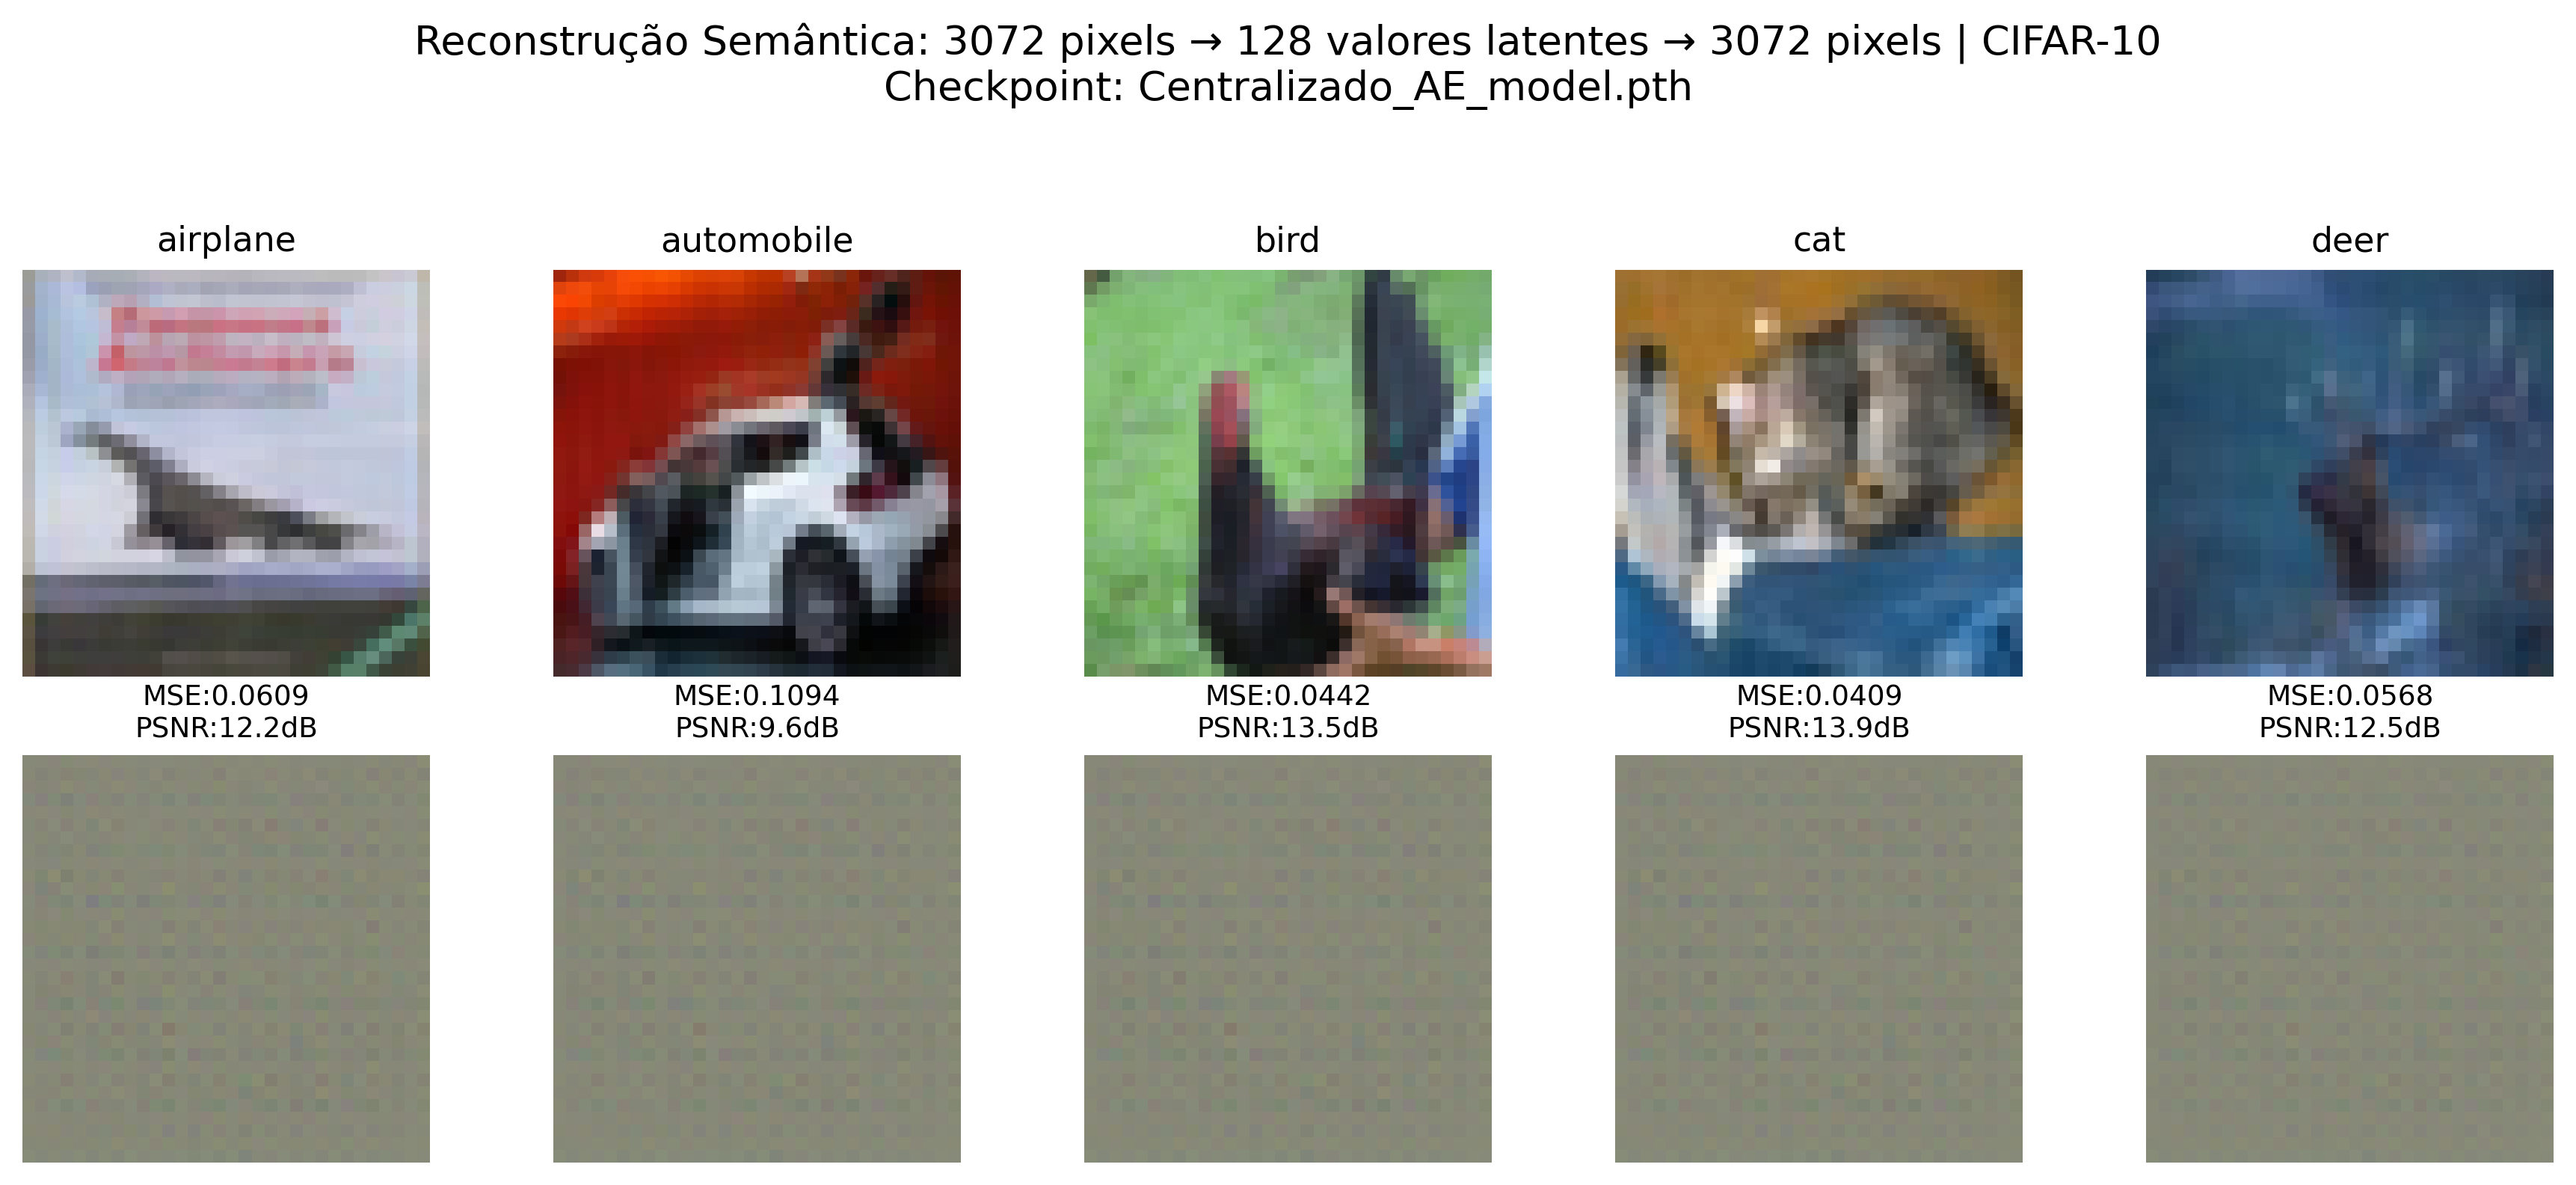
\includegraphics[width=\linewidth]{figures/fig_reconstruction.png}
\caption{Exemplos de imagens originais (topo) e reconstruções semânticas (base) geradas pelo autoencoder treinado federadamente. Abaixo de cada reconstrução, MSE e PSNR individuais.}
\label{fig:reconstruction}
\end{figure}

\input{tables/tab_reconstruction}

A Tabela~\ref{tab:reconstruction} confirma que o autoencoder preserva a informação semântica com MSE médio de 0,073 e PSNR médio de 11,6~dB. Os dígitos mais simples, como o ``1'' (MSE = 0,035, PSNR = 14,6~dB), são reconstruídos com maior fidelidade, enquanto dígitos com traços mais complexos, como o ``3'' (MSE = 0,111, PSNR = 9,5~dB), apresentam maior erro. Apesar da compressão agressiva de 24,5$\times$, todos os dígitos permanecem claramente reconhecíveis, confirmando a viabilidade da comunicação semântica.

\subsection{Eficiência da Compressão Semântica}

A principal vantagem da comunicação semântica é a redução drástica no volume de dados transmitidos. A Tabela~\ref{tab:compression} compara o custo de transmissão entre a abordagem tradicional (envio da imagem completa) e a abordagem semântica (envio do vetor latente).

\begin{table}[h]
\centering
\caption{Comparação de custos de transmissão}
\label{tab:compression}
\begin{tabular}{lrr}
\toprule
\textbf{Método} & \textbf{Dados} & \textbf{Bytes} \\
\midrule
Imagem completa (raw) & 784 pixels & 3.136 B \\
Imagem PNG comprimida & --- & $\sim$300 B \\
Vetor latente (semântico) & 32 valores & 128 B \\
\bottomrule
\end{tabular}
\end{table}

\noindent O vetor latente de 32 valores float32 ocupa apenas 128 bytes, contra 3.136 bytes da imagem raw (pixels float32) — uma redução de \textbf{24,5 vezes}. Mesmo comparado com compressão PNG tradicional, a representação semântica é mais de 2$\times$ mais eficiente, com a vantagem adicional de que o receptor pode reconstruir a imagem completa a partir desses 128 bytes.

\subsection{Teste de Completação de Imagens Parciais}

Um aspecto particularmente relevante da comunicação semântica é a capacidade de \textit{completar informação faltante}. Neste experimento, enviamos apenas uma fração da imagem (mascarando o restante) e avaliamos se o modelo é capaz de reconstruir a imagem completa.

\begin{figure}[h]
\centering
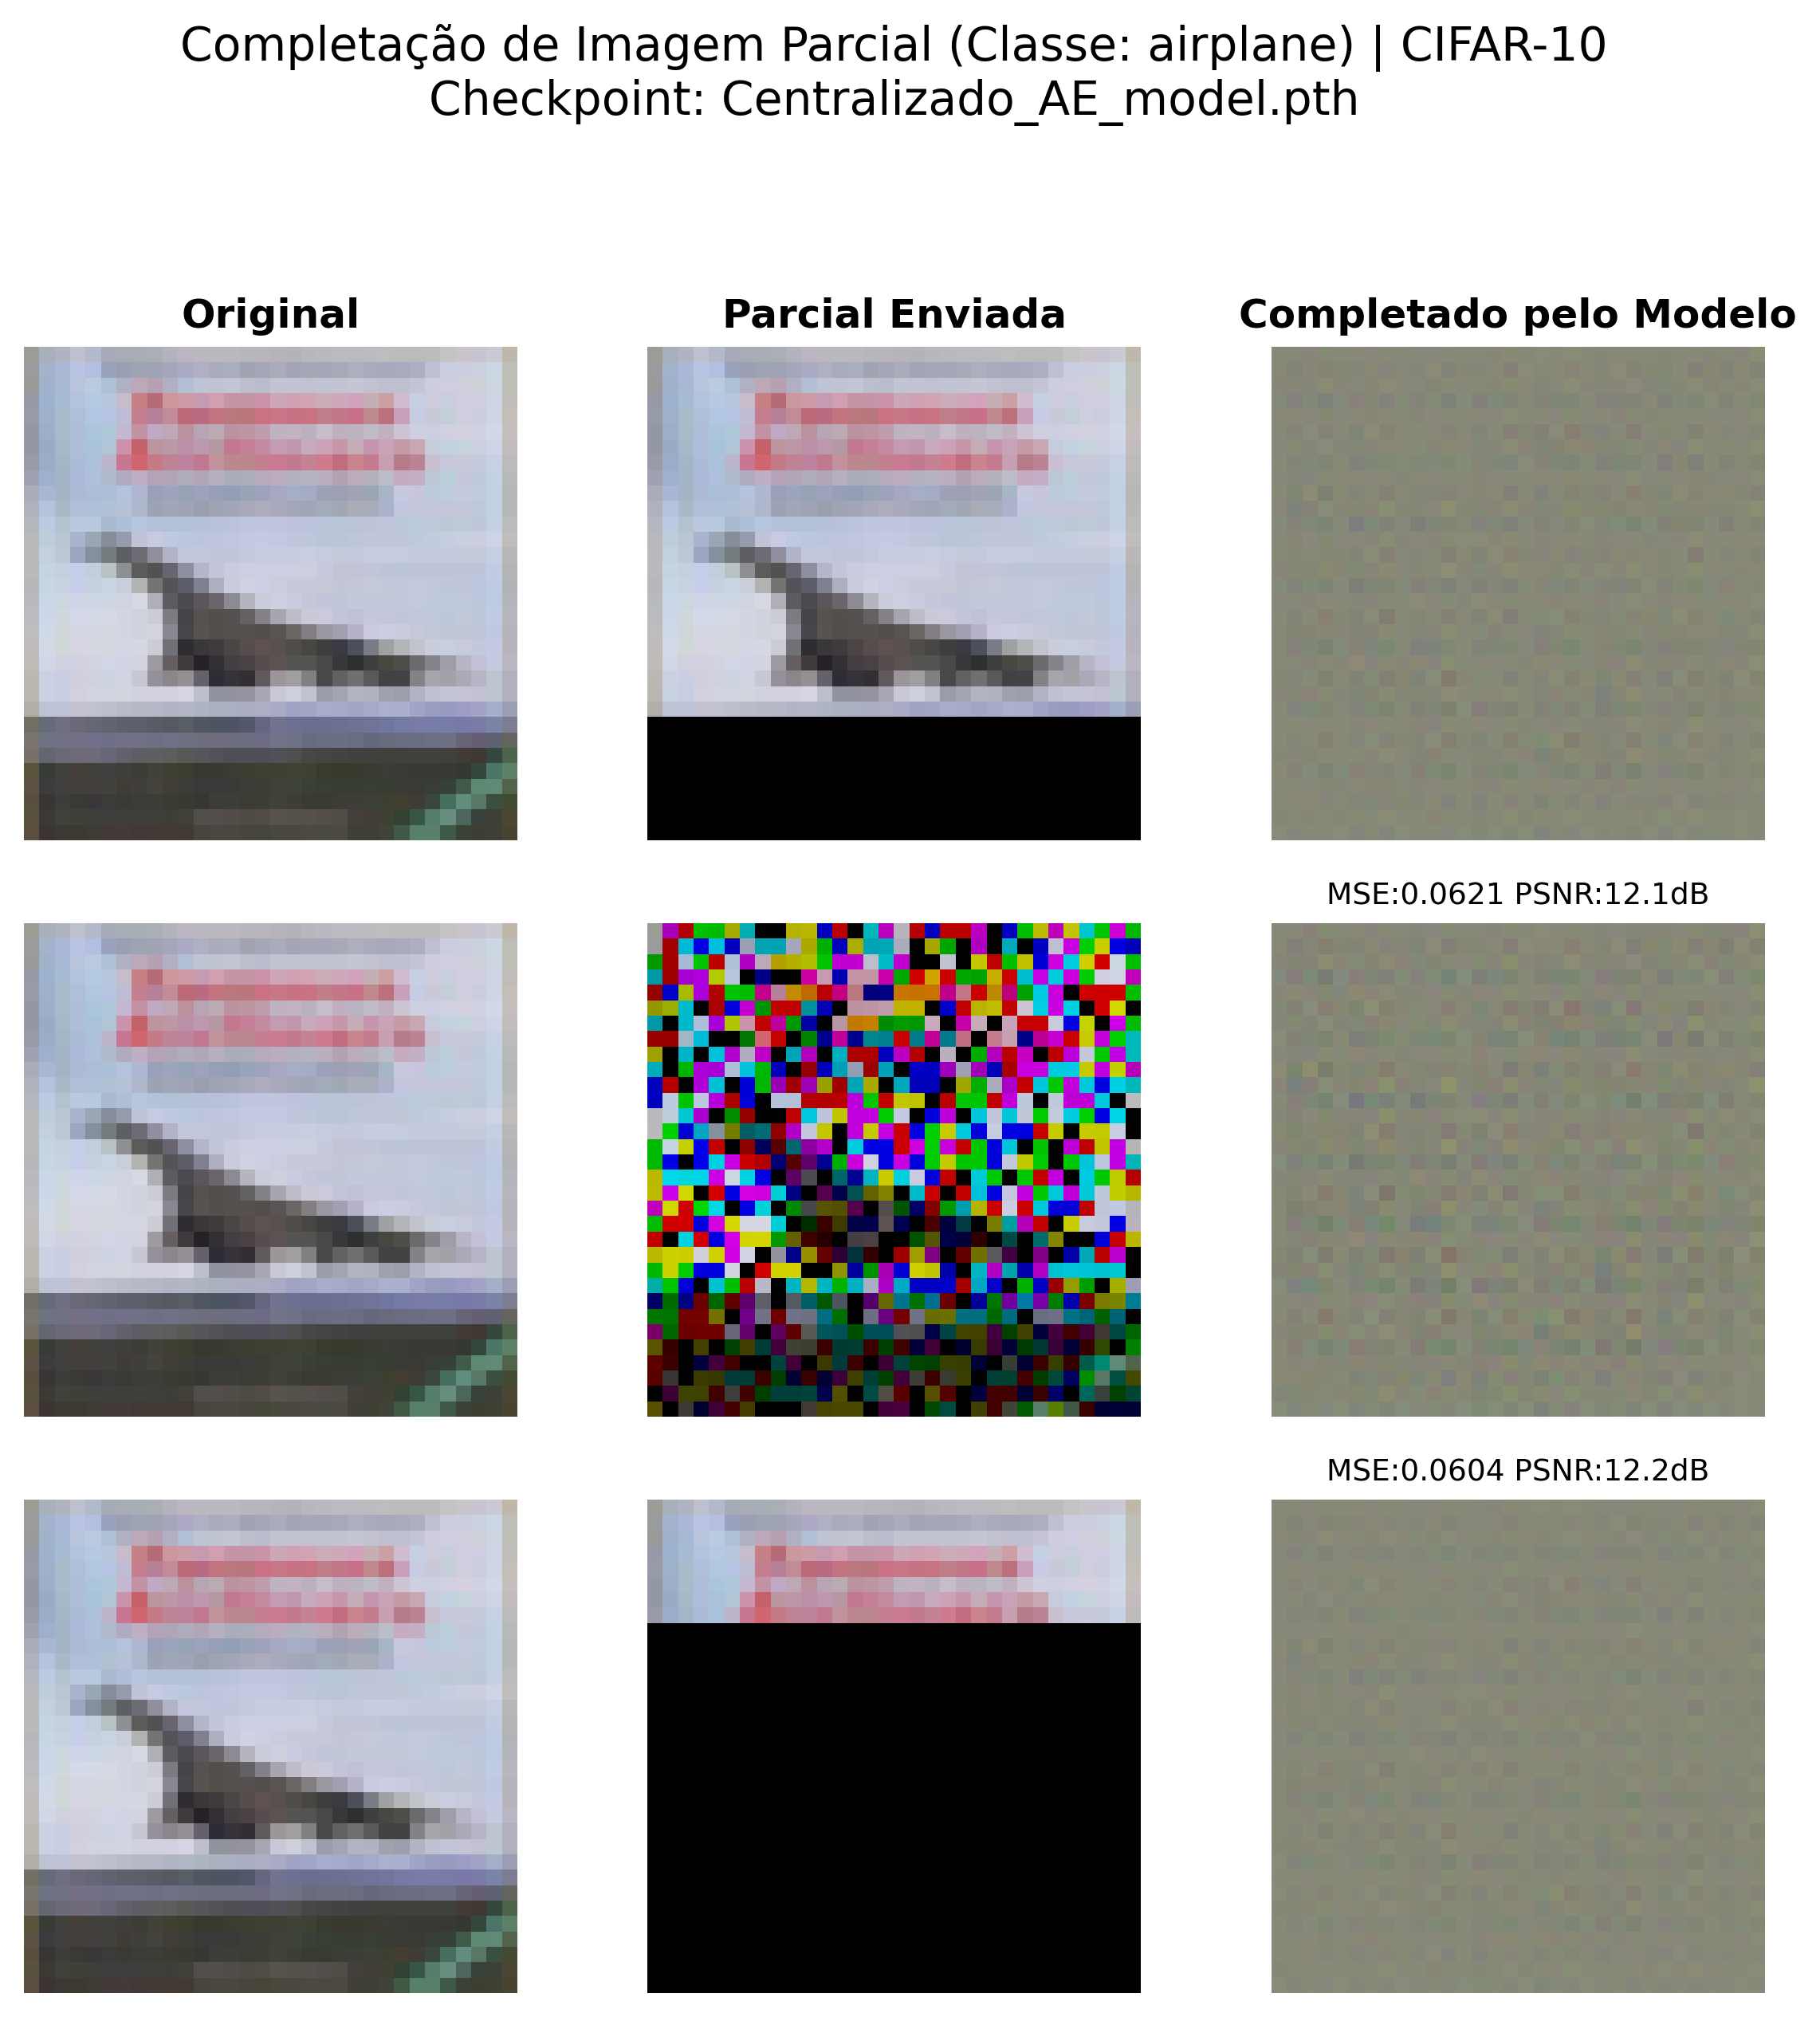
\includegraphics[width=\linewidth]{figures/fig_completion.png}
\caption{Completação de imagens parciais com diferentes níveis de mascaramento. Coluna 1: original. Coluna 2: imagem mascarada (parcial enviada). Coluna 3: reconstrução pelo autoencoder.}
\label{fig:completion}
\end{figure}

A Tabela~\ref{tab:completion} apresenta as métricas de qualidade para diferentes porcentagens de mascaramento.

\input{tables/tab_completion}

Os resultados revelam um comportamento notável: a qualidade de completação é consistente em todos os tipos e porcentagens de mascaramento, com MSE entre 0,082 e 0,090 e PSNR entre 10,5 e 10,8~dB. Essa estabilidade decorre do gargalo latente de 32 dimensões: o autoencoder já descarta mais de 95\% da informação durante a codificação, de modo que a perda adicional causada pelo mascaramento tem impacto marginal. Comparando com a reconstrução sem mascaramento (MSE médio de 0,073), a degradação máxima é de apenas 23\%, mesmo com 75\% da imagem mascarada. Isso demonstra que o modelo aprendeu uma representação semântica robusta capaz de inferir o conteúdo visual faltante.

\subsection{Impacto da Injeção de Caos}

Para avaliar a resiliência do sistema, executamos quatro cenários de injeção de caos com severidade crescente, conforme a Tabela~\ref{tab:chaos_scenarios}.

\begin{table}[h]
\centering
\caption{Cenários de injeção de caos}
\label{tab:chaos_scenarios}
\begin{tabular}{lcccc}
\toprule
\textbf{Cenário} & \textbf{Perda} & \textbf{Latência} & \textbf{Corrup.} & \textbf{Dup.} \\
\midrule
Normal & 0\% & 0 ms & 0\% & 0\% \\
Leve & 1\% & 200 ms & 0\% & 0\% \\
Moderado & 3\% & 500 ms & 0,5\% & 1\% \\
Severo & 5\% & 1000 ms & 2\% & 5\% \\
\bottomrule
\end{tabular}
\end{table}

\input{tables/tab_chaos_results}

\begin{figure}[h]
\centering
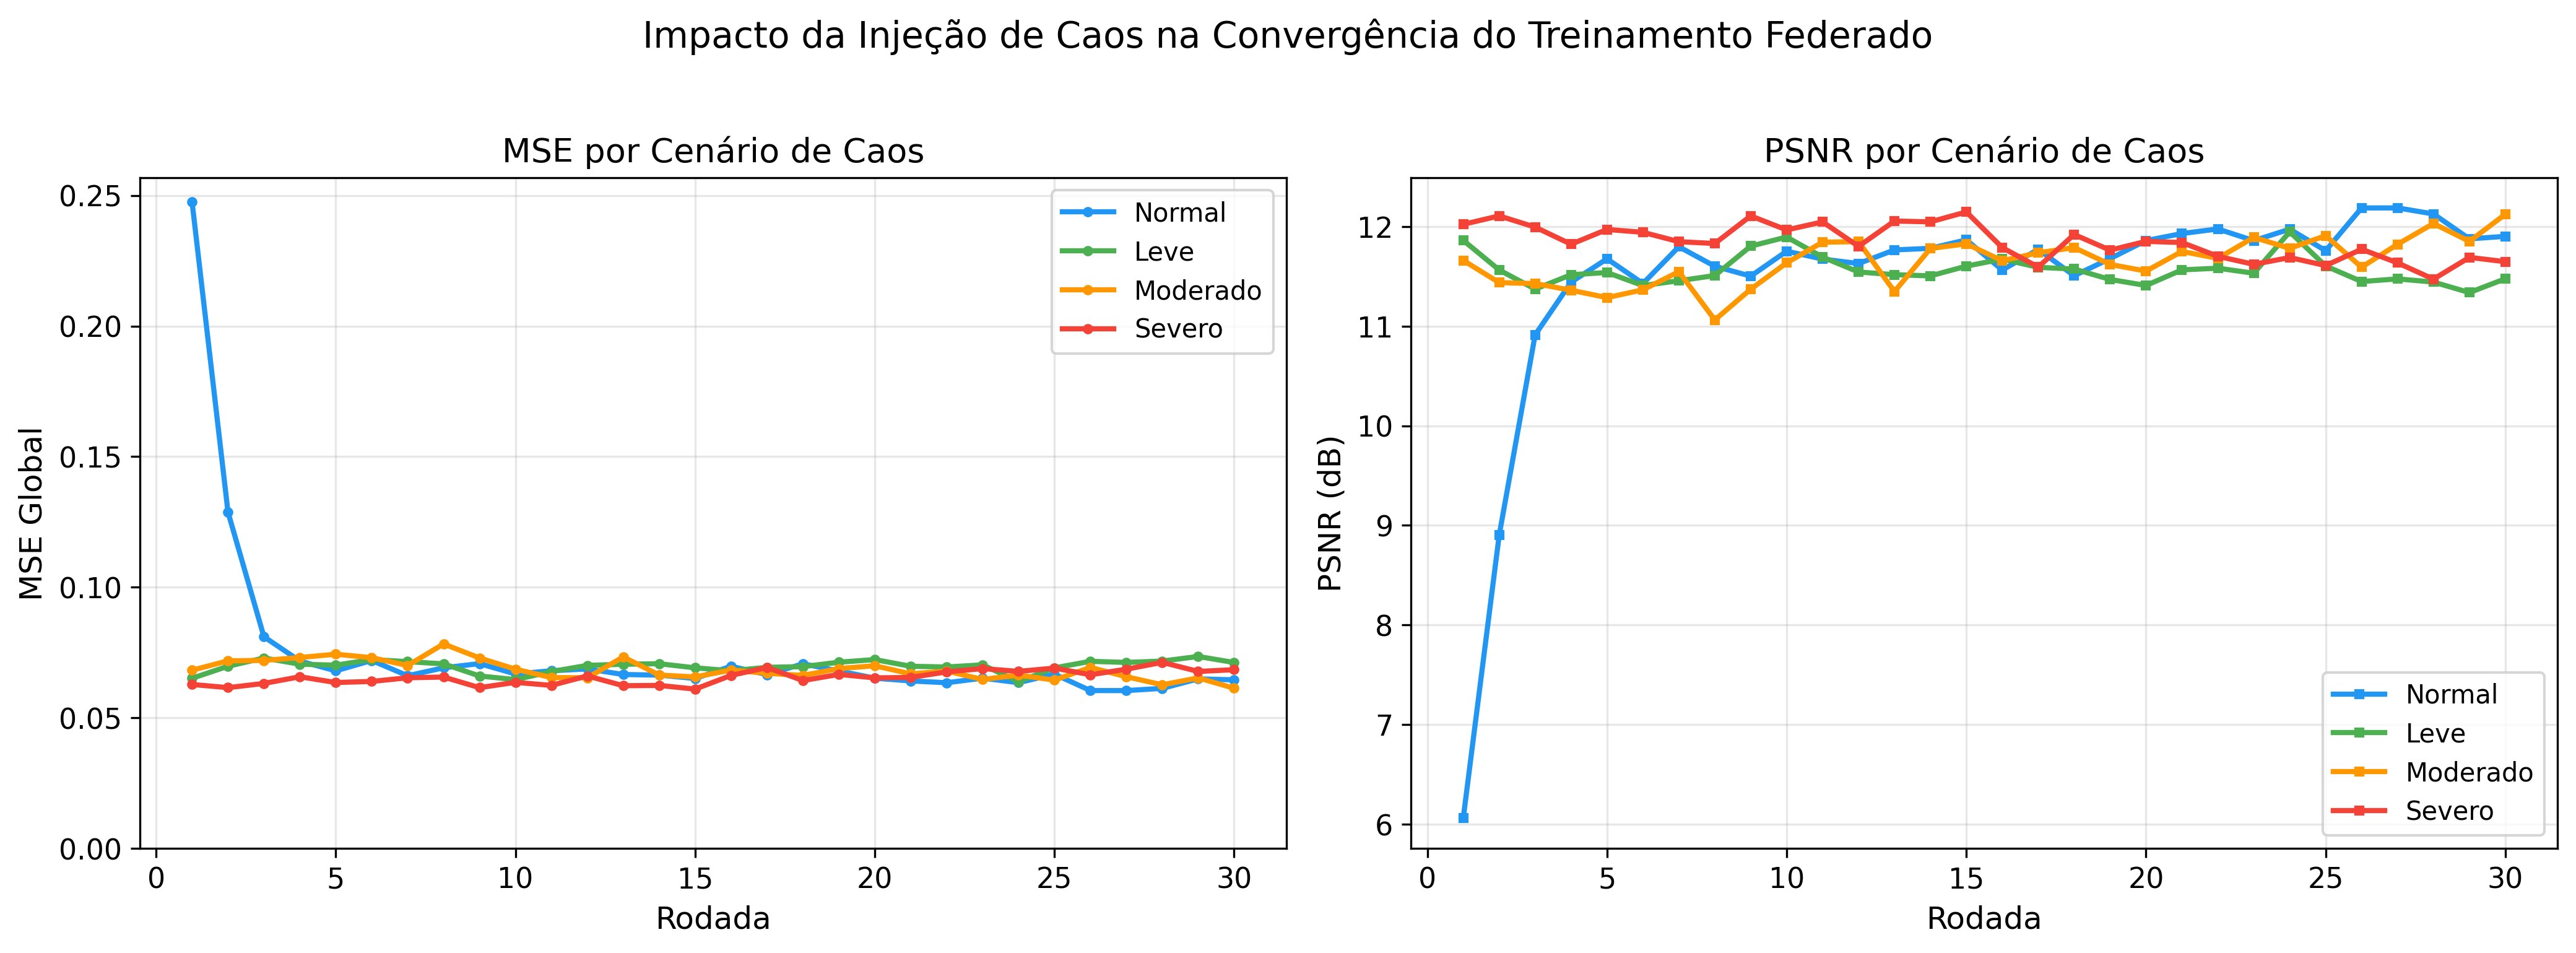
\includegraphics[width=\linewidth]{figures/fig_chaos.png}
\caption{Impacto da injeção de caos na convergência do treinamento federado. Esquerda: MSE global por rodada. Direita: PSNR global por rodada.}
\label{fig:chaos_convergence}
\end{figure}

Os resultados da Tabela~\ref{tab:chaos_results} e da Figura~\ref{fig:chaos_convergence} revelam que o framework é altamente resiliente à injeção de caos. Todos os quatro cenários convergem para qualidade semelhante: MSE final entre 0,061 e 0,071 e PSNR final entre 11,5 e 12,1~dB. O cenário Normal atinge MSE = 0,071 (PSNR = 11,5~dB), enquanto os cenários com caos atingem valores comparáveis — o cenário Moderado, inclusive, registra o melhor MSE final (0,061, PSNR = 12,1~dB). Esse resultado é explicado pelo mecanismo de timeout implementado no servidor: quando o cliente instável falha em entregar pesos dentro de 30 segundos, o servidor agrega com os clientes disponíveis, garantindo progresso contínuo. A principal diferença observada é no tempo de convergência: o cenário Normal completa 30 rodadas em aproximadamente 3 minutos, enquanto o cenário Severo requer cerca de 22 minutos devido à latência de 1000~ms e às falhas intermitentes.

\subsection{Comparação: Treinamento Federado vs. Centralizado}

Para quantificar o custo do treinamento distribuído em termos de qualidade do modelo, comparamos o treinamento federado (FedAvg com 3 clientes) com o treinamento centralizado (todos os dados em um único nó), utilizando os mesmos hiperparâmetros e número de rodadas. A Tabela~\ref{tab:fl_vs_central} apresenta os resultados.

\begin{table}[ht]
\centering
\caption{Comparação Federado vs. Centralizado (30 rodadas)}
\label{tab:fl_vs_central}
\begin{tabular}{lccc}
\toprule
\textbf{Configuração} & \textbf{MSE} & \textbf{PSNR (dB)} & \textbf{SSIM} \\
\midrule
Centralizado AE & 0,0576 & 12,4 & 0,563 \\
Centralizado VAE & 0,0655 & 11,8 & 0,466 \\
FL AE (FedAvg, 3 clients) & 0,0708 & 11,5 & --- \\
\bottomrule
\end{tabular}
\end{table}

O treinamento centralizado AE atinge MSE 18,6\% menor que o FL AE (0,058 vs. 0,071), confirmando o trade-off esperado: o FL sacrifica qualidade em favor de privacidade e descentralização. O VAE centralizado apresenta MSE levemente superior ao AE centralizado (0,066 vs. 0,058), o que se explica pelo termo de regularização KL na função de perda — o VAE ``gasta'' parte de sua capacidade organizando o espaço latente, o que reduz a fidelidade pixel a pixel mas habilita capacidades generativas.

\subsection{Discussão}

Os resultados permitem uma análise integrada dos componentes do framework à luz das referências:

\textbf{Comunicação Semântica e Compressão.} A compressão de 96\% alcança MSE médio de 0,073 (PSNR 11,6~dB), suficiente para preservar a informação semântica dos dígitos. Dígitos simples como o ``1'' (MSE=0,035, PSNR=14,6~dB) são reconstruídos com alta fidelidade, enquanto dígitos com geometria complexa (``3'', ``8'') apresentam maior erro. Comparado com a compressão PNG tradicional ($\sim$300 bytes), a representação semântica (128 bytes) é mais de 2$\times$ mais eficiente.

\textbf{AE vs. VAE.} O AE determinístico supera o VAE em métricas de reconstrução pura (MSE, PSNR), como esperado — o termo KL do VAE regulariza o espaço latente ao custo de fidelidade pixel a pixel. Entretanto, o VAE oferece capacidades únicas: geração de novas amostras por amostragem de $\mathbf{z} \sim \mathcal{N}(\mathbf{0}, \mathbf{I})$, espaço latente contínuo para interpolação, e maior robustez teórica a perturbações no canal \cite{grassucci2023genai_meets_semcom}. Esse trade-off reflete o dilema identificado por Higgins et al. \cite{higgins2017beta_vae}: o $\beta$-VAE permite ajustar explicitamente o equilíbrio entre reconstrução e regularidade.

\textbf{FL vs. Centralizado.} A degradação de 18,6\% no MSE do FL em relação ao centralizado é o preço da privacidade. O FedAvg converge mesmo com dados non-IID e compressão Top-K agressiva, confirmando sua robustez. O mecanismo de timeout com agregação parcial garante progresso mesmo sob falhas.

\textbf{Resiliência ao Caos.} Os quatro cenários convergem para qualidade semelhante (MSE 0,061--0,071), demonstrando que o mecanismo de aggregação parcial por timeout é efetivo. A principal diferença é temporal: o cenário Severo requer $\sim$7$\times$ mais tempo que o Normal.

\textbf{Relação com o Estado da Arte.} Nosso framework aborda lacunas identificadas nas referências: (i) implementamos um modelo genuinamente generativo (VAE) conforme proposto por Grassucci et al. \cite{grassucci2023genai_meets_semcom}; (ii) simulamos canal AWGN no espaço latente, aproximando-se do conceito de JSCC de Bourtsoulatze et al. \cite{bourtsoulatze2019deep}; (iii) avaliamos com SSIM \cite{wang2004ssim}, métrica padrão recomendada; e (iv) demonstramos a viabilidade de treinar codecs semânticos generativos via FL em um testbed prático, respondendo à necessidade apontada por Luo et al. \cite{luo2022semantic}.

\textbf{Limitações.} O dataset MNIST (28$\times$28, 1 canal) é relativamente simples; extensão para imagens coloridas e de maior resolução é necessária. O número de clientes (3) é limitado. A simulação de canal AWGN no espaço latente é uma aproximação do canal wireless real. O SSIM obtido ($\sim$0,5) indica preservação semântica mas não perfeição visual, o que é esperado dada a compressão agressiva de 96\%.


% ========================
% SEÇÃO 5: CONCLUSÃO E TRABALHOS FUTUROS
% ========================
\section{Conclusão e Trabalhos Futuros}
\label{sec:conclusion}

Este trabalho apresentou um framework containerizado para comunicação semântica de imagens baseado em aprendizado federado e IA generativa. O sistema integra dois modelos — um autoencoder determinístico e um VAE generativo \cite{kingma2014vae} — treinados de forma distribuída via FedAvg com três clientes de perfis distintos (estável, instável com Top-K 60\%, e heterogêneo Non-IID). Ambos os modelos comprimem imagens MNIST de 784 pixels para 32 valores latentes (redução de 96\%), com o AE atingindo MSE = 0,071 (federado) e o centralizado atingindo MSE = 0,058 — evidenciando o trade-off privacidade vs. qualidade inerente ao FL. O VAE, além de comprimir e reconstruir, habilita a geração de novas imagens por amostragem do espaço latente, justificando o componente de IA generativa.

Os experimentos demonstram: (i) resiliência sob quatro cenários de caos (MSE 0,061--0,071 em todos), com o mecanismo de timeout garantindo convergência mesmo sob 5\% de perda e 1000~ms de latência; (ii) capacidade de completação de imagens parciais com degradação máxima de 23\% mesmo com 75\% da imagem mascarada; (iii) viabilidade de treinar codecs semânticos generativos via FL em um testbed prático e reprodutível baseado em Docker.

Para trabalhos futuros, identificamos as seguintes direções:

\begin{itemize}[leftmargin=*]
    \item Extensão para datasets complexos (CIFAR-10, imagens médicas) com arquiteturas mais profundas (ResNet-VAE);
    \item Integração de modelos de difusão como codec semântico, conforme proposto por Du et al. \cite{du2023genai_semcom};
    \item Compressão adaptativa ao canal \cite{xia2023gennet_layer}, com dimensão latente e $\beta$-VAE ajustáveis dinamicamente conforme SNR;
    \item Escalabilidade para 10+ clientes com esquemas de agregação robustos (Krum, Trimmed Mean) contra clientes bizantinos;
    \item Incorporação de métricas perceptuais avançadas (LPIPS, FID) e avaliação em canais com desvanecimento (Rayleigh fading).
\end{itemize}

% ========================
% REFERÊNCIAS
% ========================
\bibliographystyle{IEEEtran}
\bibliography{ref}

\end{document}
